\chapter{Radzenie sobie z opresją}
\AddToShipoutPictureBG*{
\includegraphics[width=\paperwidth,height=\paperheight]{TeX_files/3-0.png}}
Artist: Mohammed Fayaz
\newpage

\begin{figure}[h]
\centering
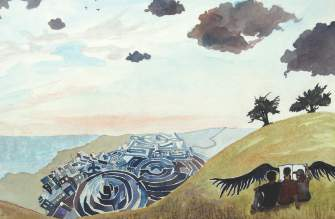
\includegraphics[width=16cm]{TeX_files/3-1.png}
\caption{Artist: Jacks McNamara}
\label{3-1}
\end{figure}

\noindent\textcolor{ProcessBlue}{\textbf{\Large{Jak sobie radzisz z wpływem opresji?}}}\\
\begin{multicols}{2}
\begin{checkboxlist}
\item Przyjaciele
\item Ćwiczenia
\item Zdrowe odżywianie
\item Joga
\item Kreatywna ekspresja
\item Jazda na rowerze - [Bicycling]
\item Rozciąganie się
\item Walcząć z opresją!
\item Aktywizm!
\item Medytacja
\item Śmiech. Zawsze śmiech
\item Korzystając z portali społecznościowych
\item Śpiew
\item Rysowanie
\item Sztuki walki
\item Natura
\item Icarus
\item Pisanie
\item Bycie częścią społeczności - Being part of a community
\item Learn about it
\item Pray for guidance
\item Nie poddając się
\item Knowing that I am not broken!
\item Peer counseling
\item Owning my opinions
\item Humor
\item Intellectualizing it
\item Współczucie
\item Pomaganie innym
\item Czytanie
\item Zabawa ze zwierzęciem
\item Chodzenie na siłownie
\item Praktyki duchowe
\item Terapia
\item Homeopatia
\item Bodywork
\item Cuddling
\item Routine
\item Otwarcie o tym mówiąć
\item Rzeźba
\item Taniec
\item Film
\item Photography
\item Solidarność z innymi
\item Sztuka
\item Muzyka
\item Picking my battles
\item Trying to take care of myself
\item Ucząć się
\item Myśląć
\item Breaking stereotypes
\item Doing things that make me happy
\item Speaking my mind
\item Pozytywne relacje
\item Admitting when I’m not okay
\item Taking a stand
\item Educating myself
\item Ograniczająć wystawianie się na opresję - [Limiting exposure to oppressor]
\item Strengthening my personal love
\item I developed talking points
\item Advocacy
\item Being open about my challenges
\item Reading empowering statements, essays, and poems
\item Organizująć się
\item Edukując innych
\item Ucząć się mówić "nie"
\item Unafraid to tell the “truth” as I see it
\item Power of Positive Thinking \& Action
\item Communicating to others
\item Having a chosen family
\item Contextualizing behavior within systemic violence so it is less shameful
\item Seeing a counselor.
\item Allowing ourselves to cry
\item Reading about other people who experience oppression in order not to feel alone
\item Going to rallies
\item Pisząć
\item Listening to cheerful music
\item Reminding ourselves that not everyone will treat us poorly
\item Reminding ourselves that the oppressors are at fault, not us
\item Acknowledge the feeling, experiencing it in our bodies, and then, after a time, try to let it go
\item Take deep breaths
\item Turning feelings into action: finding a healthy venue for all the passion and emotional work that needs to be done
\item Escapism into a book or a TV show is nice
\item Meditate on simplicity and non-violent solutions
\item Taking a stand
\item Developing a good relationship with a trusted healthcare provider
\item Allow ourselves to take a day or two to recover
\item Remembering that life is not a race
\item Reiki
\item Detox
\item Ćwiczenia
\item Being in nature
\item Opiekując się zwierzętami Caring for animals
\item Nurturing people
\item Bycie przyjacielem i nauczycielem dal innych
\item Pisanie i czytanie
\item Sztuka
\item Wyrażaniw tego co niewyrażalne
\item Wyżycie się/ Wyładowywanie się
\item Przypomnienie sobie żę kochamy życie - Reminding ourselves that we love life
\item Praktyki duchowe
\item Robienir czegoś więcej niż egzystowanie - [Doing more rather than just existing]
\item Zaangażowanie w troszczenie się o siebie - [Engage in self care]
\item Sięganie po pomoc
\item Głęboki oddech
\item Mówienie di siebie
\item Ćwiczenia
\item Sen
\end{checkboxlist}
\end{multicols}

\newpage
\begin{figure}[h]
\centering
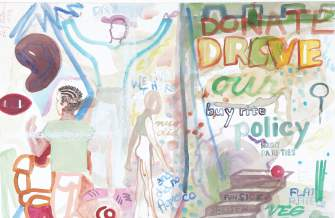
\includegraphics[width=16cm]{TeX_files/3-2.png}
\caption{Artist: Eddy Falconer}
\label{3-2}
\end{figure}

\noindent\textcolor{ProcessBlue}{\textbf{\Large{Jak jeszcze inaczej możesz radzić sobie z wpływem opresji?}}}\\
\noindent\rule{\textwidth}{1pt}\\
\noindent\rule{\textwidth}{1pt}\\
\noindent\rule{\textwidth}{1pt}\\
\noindent\rule{\textwidth}{1pt}\\
\noindent\rule{\textwidth}{1pt}\\
\noindent\rule{\textwidth}{1pt}\\
\noindent\rule{\textwidth}{1pt}\\
\noindent\rule{\textwidth}{1pt}\\
\noindent\rule{\textwidth}{1pt}\\
\noindent\rule{\textwidth}{1pt}\\
\noindent\rule{\textwidth}{1pt}\\
\noindent\rule{\textwidth}{1pt}\\
\noindent\rule{\textwidth}{1pt}\\
\noindent\rule{\textwidth}{1pt}\\\\

\newpage
\noindent\textcolor{ProcessBlue}{\textbf{\Large{Jak radzisz sobie z sytuacjami prowokującymi opresję?}}}\\
\begin{figure}[h]
\centering
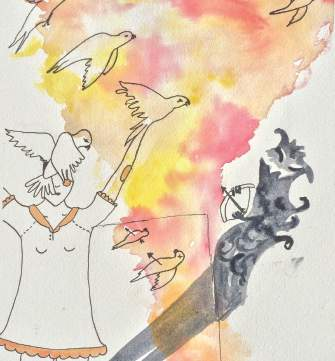
\includegraphics[width=17cm]{TeX_files/3-3.png}
\caption{Artist: Jess Rankine}
\label{3-3}
\end{figure}

\begin{checkboxlist}
\item Try to stay cool
\item Detach as quickly as possible
\item Listen to peaceful music
\item Malująć
\item Advise the person who triggered the sensation that you need to take a moment and, say, get a glass of water
\item Reach out to others if you feel too overwhelmed
\item Let people know how they are affecting you
\item Disengage or go for a walk
\item Recognize where the anxiety is coming from
\item Stay in your comfort zone with the people you know until you find someone trusted you can confide in
\end{checkboxlist}

\noindent\textcolor{ProcessBlue}{\textbf{\Large{What helps you navigate triggering situations?}}}
\noindent\textcolor{ProcessBlue}{\textbf{\Large{How can others help you?}}}\\
\noindent\rule{\textwidth}{1pt}\\
\noindent\rule{\textwidth}{1pt}\\
\noindent\rule{\textwidth}{1pt}\\
\noindent\rule{\textwidth}{1pt}\\
\noindent\rule{\textwidth}{1pt}\\
\noindent\rule{\textwidth}{1pt}\\
\noindent\rule{\textwidth}{1pt}\\
\noindent\rule{\textwidth}{1pt}\\
\noindent\rule{\textwidth}{1pt}\\
\noindent\rule{\textwidth}{1pt}\\
\noindent\rule{\textwidth}{1pt}\\
\noindent\rule{\textwidth}{1pt}\\
\noindent\rule{\textwidth}{1pt}\\
\noindent\rule{\textwidth}{1pt}\\
\noindent\rule{\textwidth}{1pt}\\
\noindent\rule{\textwidth}{1pt}\\
\noindent\rule{\textwidth}{1pt}\\
\noindent\rule{\textwidth}{1pt}\\\
\newpage

\noindent\textcolor{ProcessBlue}{\textbf{\Large{Jak inni ludzie mogą ci pomóc?}}}
\noindent\textcolor{ProcessBlue}{\textbf{\Large{Jak możemy sobie pomóc na wzajem??}}}\\
\begin{multicols}{2}
\begin{checkboxlist}
\item Nie mów mi: "Otrząśnij się z tego" albo "Wszystko będzie dobrze"
\item Zrób mi herbatę
\item Przynieś mi kwiaty
\item Nie ignoruj mnie
\item Pokaż mi że mnie kochasz
\item Normalize my feelings
\item Przyłąćz się do mnie w działaniu
\item Validate me
\item Wierz
\item Name the oppression
\item Make connections with others who have similar experiences
\item Validate my experience
\item Normalize
\item Listen to me
\item Say it is not okay
\item Don’t try to fix me
\item Help me up to a better plane of existence
\item Be present
\item Run me a bath
\item Hear and acknowledge the experience
\item Getting me comfy clothes to change into
\item Distract me
\item Tell me a joke or share funny stories
\item Watch a movie with me
\item Talk to me about superficial topics, like celebrities or popular culture
\item Don’t discourage my dreams
\item Believe I am capable of anything despite my struggles and obstacles
\item Educate yourself
\item Help me focus on the things I like
\item Acknowledge that you are capable of racist acts without being racist
\item Appreciate my voice
\item Don’t tell me how I feel
\item Be an ear, even if you don’t agree with me
\item Speak about positive things
\item Engage in intellectual debate
\item Invite me to get together
\item Don’t shoot down my ideas
\item Come visit
\item Treat me like an adult
\item Bring over a treat
\item Tell me that you love me regardless of what happens to me
\item Remembering that it takes me time to heal
\item Stay with me
\item Don’t pressure me
\item Give me space
\item Accept my feelings
\item Be aware
\item Don’t give unsolicited advice
\item Miej cierpliwość/Bądź cierpliwy
\item Przypomnij mi o rzeczach które pomogły mi w przeszłości
\item Bądź wyrozumiały
\item Okaż współczucie
\item Ni mów ,"Dobrze wiem jak się czujesz" - [Don’t say, “I know exactly how you feel”]
\item Przypomnij mi o moich umiejętnościach - [Remind me of my skills]
\item Przytul mnie
\item Pomósz mi użyć moich umiejętności - [Help me use some my skills]
\item Wierz w to co mówię
\item Bądź przy mnie
\item Trzymaj mnie za rękę
\item Nie porzucaj mnie
\item Zaoferuj telefon do mojego terapeuty w moim imieniu - [Offer to call my therapist for me]
\item Pomóż mi redukując napięcie
\item Zaproponuj zajęcie się sprawami - [Offer to run errands]
\end{checkboxlist}
\end{multicols}
\noindent\textcolor{ProcessBlue}{\textbf{\Large{In what other ways can people help you?}}}
\noindent\textcolor{ProcessBlue}{\textbf{\Large{What is helpful? What isn’t?}}}\\
\noindent\rule{\textwidth}{1pt}\\
\noindent\rule{\textwidth}{1pt}\\
\noindent\rule{\textwidth}{1pt}\\
\noindent\rule{\textwidth}{1pt}\\
\noindent\rule{\textwidth}{1pt}\\
\noindent\rule{\textwidth}{1pt}\\
\noindent\rule{\textwidth}{1pt}\\
\noindent\rule{\textwidth}{1pt}\\
\noindent\rule{\textwidth}{1pt}\\
\noindent\rule{\textwidth}{1pt}\\
\noindent\rule{\textwidth}{1pt}\\\\
\newpage
\noindent\rule{\textwidth}{1pt}\\
\noindent\rule{\textwidth}{1pt}\\
\noindent\rule{\textwidth}{1pt}\\
\noindent\rule{\textwidth}{1pt}\\
\noindent\rule{\textwidth}{1pt}\\
\noindent\rule{\textwidth}{1pt}\\
\noindent\rule{\textwidth}{1pt}\\
\noindent\rule{\textwidth}{1pt}\\
\noindent\rule{\textwidth}{1pt}\\
\noindent\rule{\textwidth}{1pt}\\
\noindent\rule{\textwidth}{1pt}\\
\noindent\rule{\textwidth}{1pt}\\
\noindent\rule{\textwidth}{1pt}\\
\noindent\rule{\textwidth}{1pt}\\
\noindent\rule{\textwidth}{1pt}\\
\noindent\rule{\textwidth}{1pt}\\
\noindent\rule{\textwidth}{1pt}\\
\noindent\rule{\textwidth}{1pt}\\
\noindent\rule{\textwidth}{1pt}\\
\noindent\rule{\textwidth}{1pt}\\
\noindent\rule{\textwidth}{1pt}\\
\noindent\rule{\textwidth}{1pt}\\
\noindent\rule{\textwidth}{1pt}\\
\noindent\rule{\textwidth}{1pt}\\
\noindent\rule{\textwidth}{1pt}\\
\noindent\rule{\textwidth}{1pt}\\\

